%%%%%%%%%%%%%%%%%%%%%%%%%%%%%%%%%%%%%%%%%%%%%%%%%%%%%%%%%%%%%%%%%%%%
%% I, the copyright holder of this work, release this work into the
%% public domain. This applies worldwide. In some countries this may
%% not be legally possible; if so: I grant anyone the right to use
%% this work for any purpose, without any conditions, unless such
%% conditions are required by law.
%%%%%%%%%%%%%%%%%%%%%%%%%%%%%%%%%%%%%%%%%%%%%%%%%%%%%%%%%%%%%%%%%%%%

\documentclass[aspectratio=169]{beamer}
\usetheme[faculty=fi]{fibeamer}
\usepackage[utf8]{inputenc}
\usepackage[
  main=spanish, %% By using `czech` or `slovak` as the main locale
                %% instead of `english`, you can typeset the
                %% presentation in either Czech or Slovak,
                %% respectively.
  english,czech, slovak %% The additional keys allow foreign texts to be
]{babel}        %% typeset as follows:
%%
%%   \begin{otherlanguage}{czech}   ... \end{otherlanguage}
%%   \begin{otherlanguage}{slovak}  ... \end{otherlanguage}
%%
%% These macros specify information about the presentation
\title{Computer Science and Computer Engineering (CS) \\ 
\small{November 12, 2020}} %% that will be typeset on the
\subtitle{Characterization of Objects in Indoor Spaces of
Human Occupation Using Knowledge Graphs } %% title page.
\author{
  Rodrigo Francisco (FI, UNAM)
}
%% These additional packages are used within the document:
\usepackage{ragged2e}  % `\justifying` text
\usepackage{booktabs}  % Tables
\usepackage{tabularx}
\usepackage{tikz}      % Diagrams
\usetikzlibrary{calc, shapes, backgrounds}
\usepackage{amsmath, amssymb}
\usepackage{url}       % `\url`s
\usepackage{listings}  % Code listings
\usepackage{multicol}
\usepackage{float}
\usepackage{wrapfig}
\usepackage{subcaption}
\graphicspath{ {assets/}{assets/beamer/}{figures/}}
\frenchspacing

\begin{document}
  \shorthandoff{-}
  \frame[c]{\maketitle}

  \begin{darkframes}
    % \section{Introducción}
    % \subsection{¿Qué es JavaScript?}
    \begin{frame}{Object Detection}
      \framesubtitle{\alert{Characteristics}}%
      Object detection has \textit{two} main tasks:
      % La detección de objetos se realiza mediante dos tareas principales:
      \begin{itemize}
        \item Image classification.
        \item Object localization.
      \end{itemize}
    \end{frame}
    
    \begin{frame}{Object Detection}
      \framesubtitle{\alert{Object localization}}%
      \begin{center}
        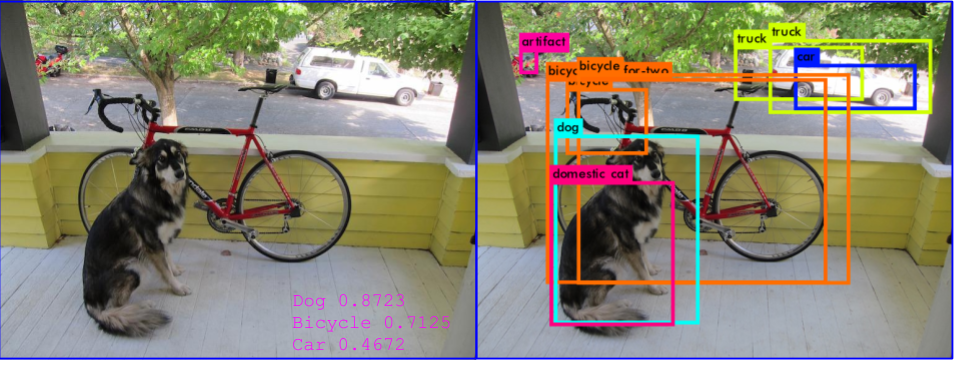
\includegraphics[width=\linewidth]{obj-loc}
      \end{center}
    \end{frame}
    
    \begin{frame}{Object detection}
      \framesubtitle{\alert{*-CNN}}%
      \begin{center}
        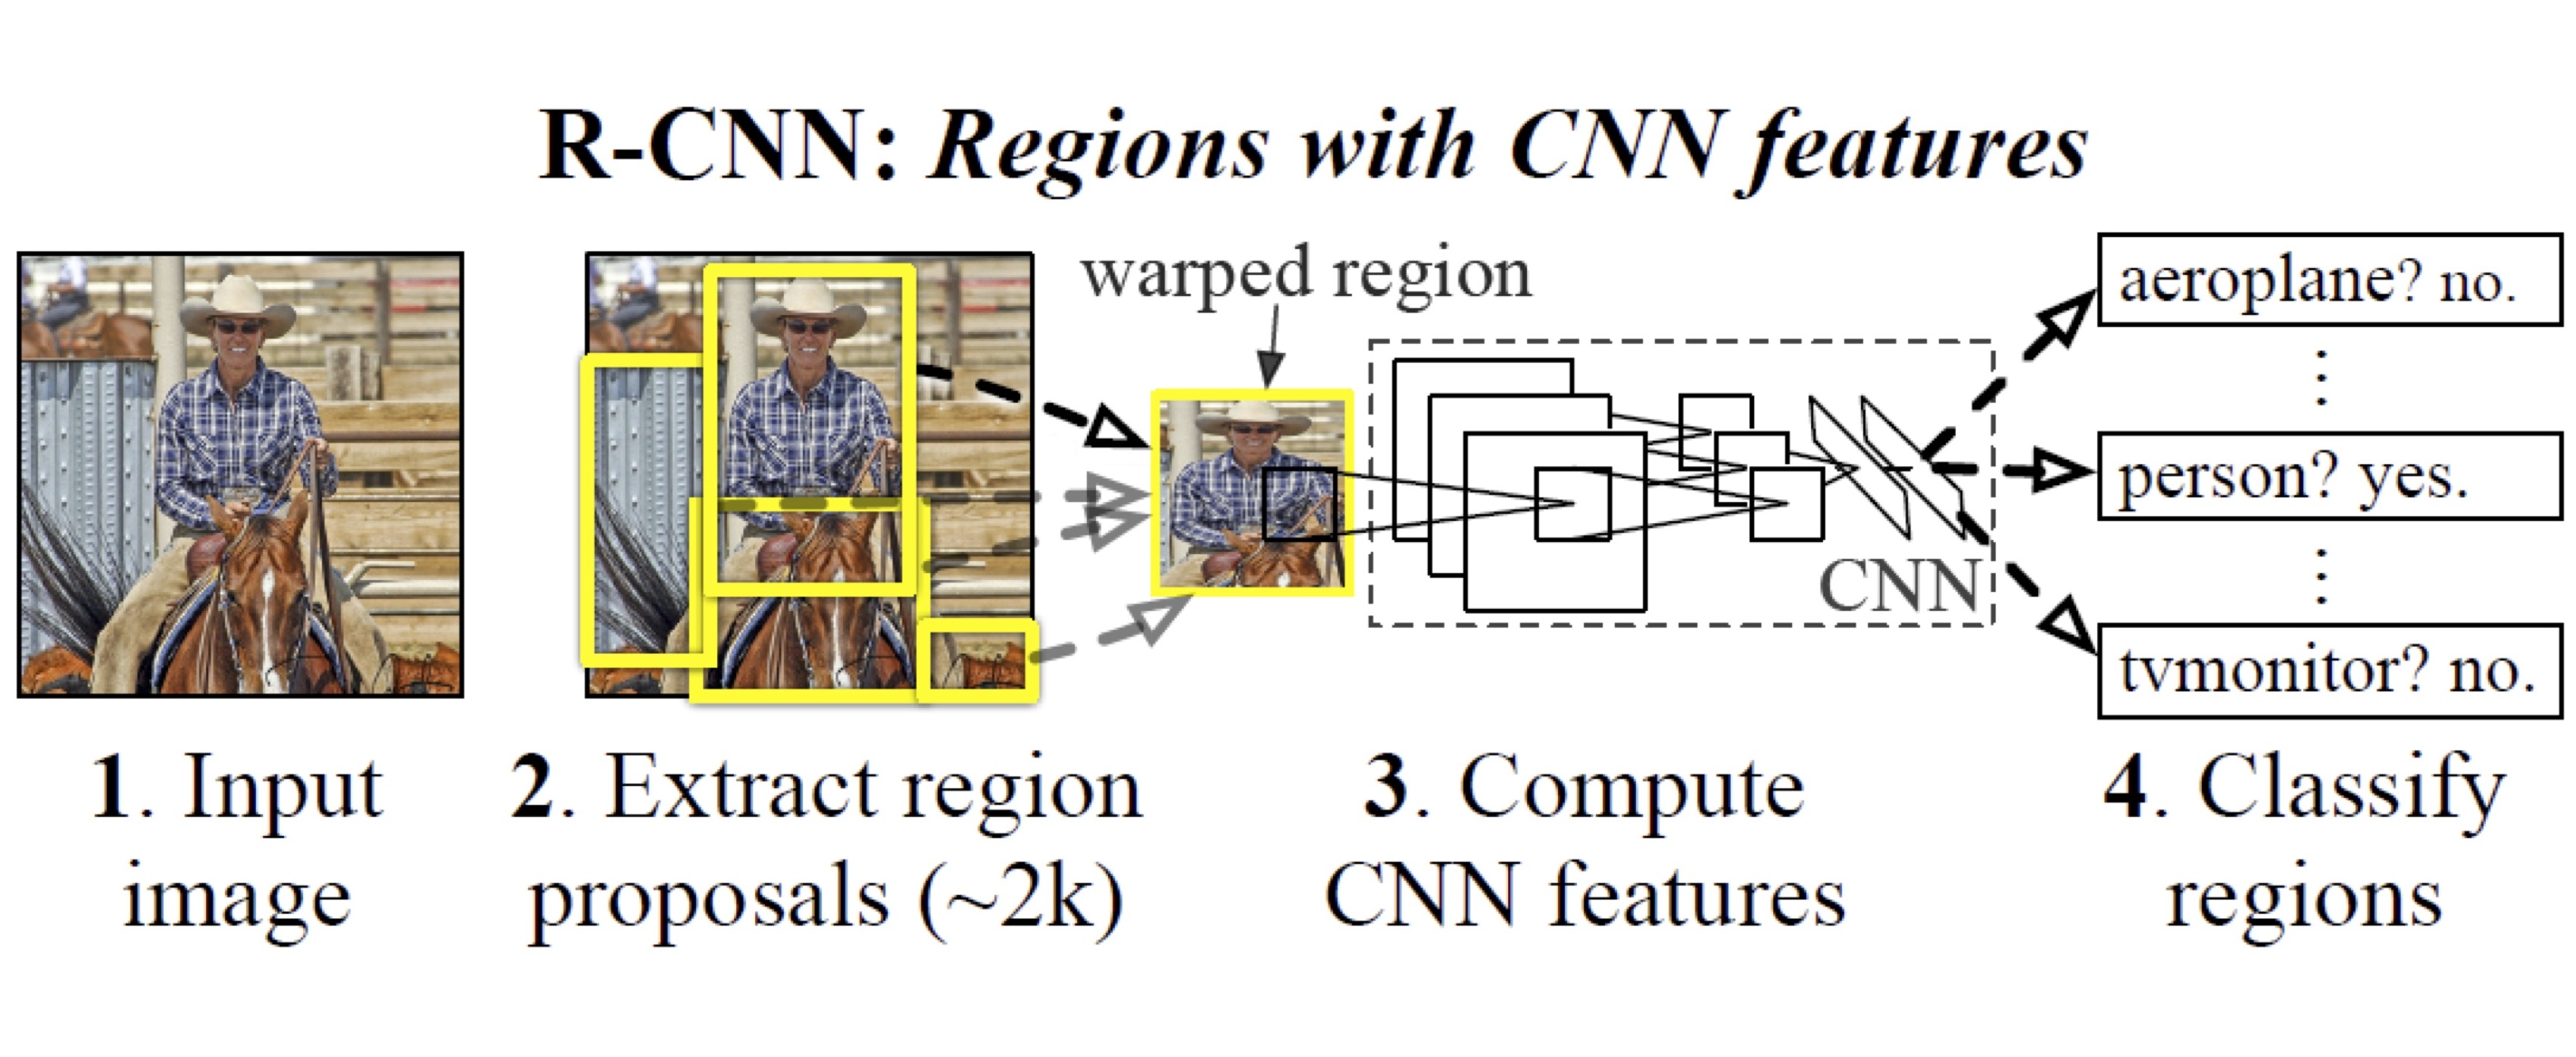
\includegraphics[width=\linewidth]{rcnn}
      \end{center}
    \end{frame}        

    \begin{frame}{Object detection}
      \framesubtitle{\alert{Convolutional Layer}}%
      \begin{center}
        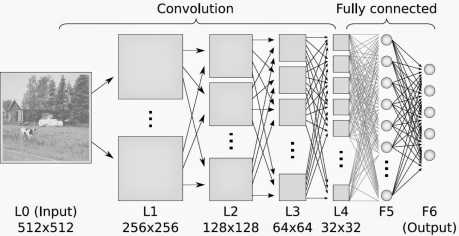
\includegraphics[width=0.8\linewidth]{conv-layer}
      \end{center}
    \end{frame}   

    \begin{frame}{Object detection}
      \framesubtitle{\alert{YOLOv2 model}}%
      \begin{center}
        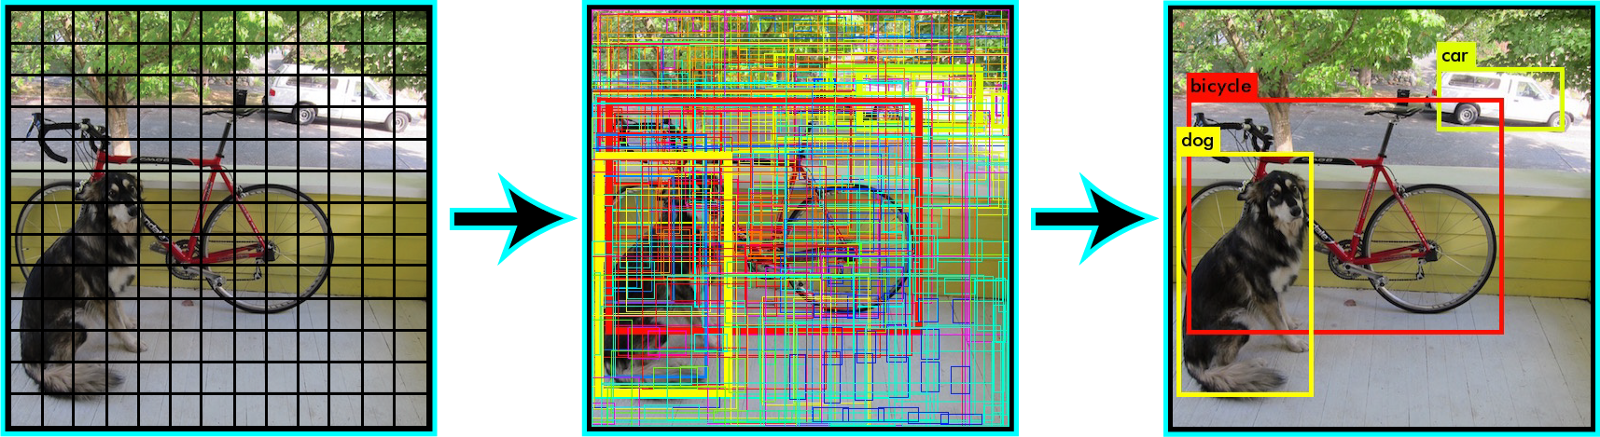
\includegraphics[width=\linewidth]{yolov2}
      \end{center}
    \end{frame}    

    \begin{frame}{Knowlegde graph}
      \framesubtitle{\alert{Example case}}%
      \begin{center}
        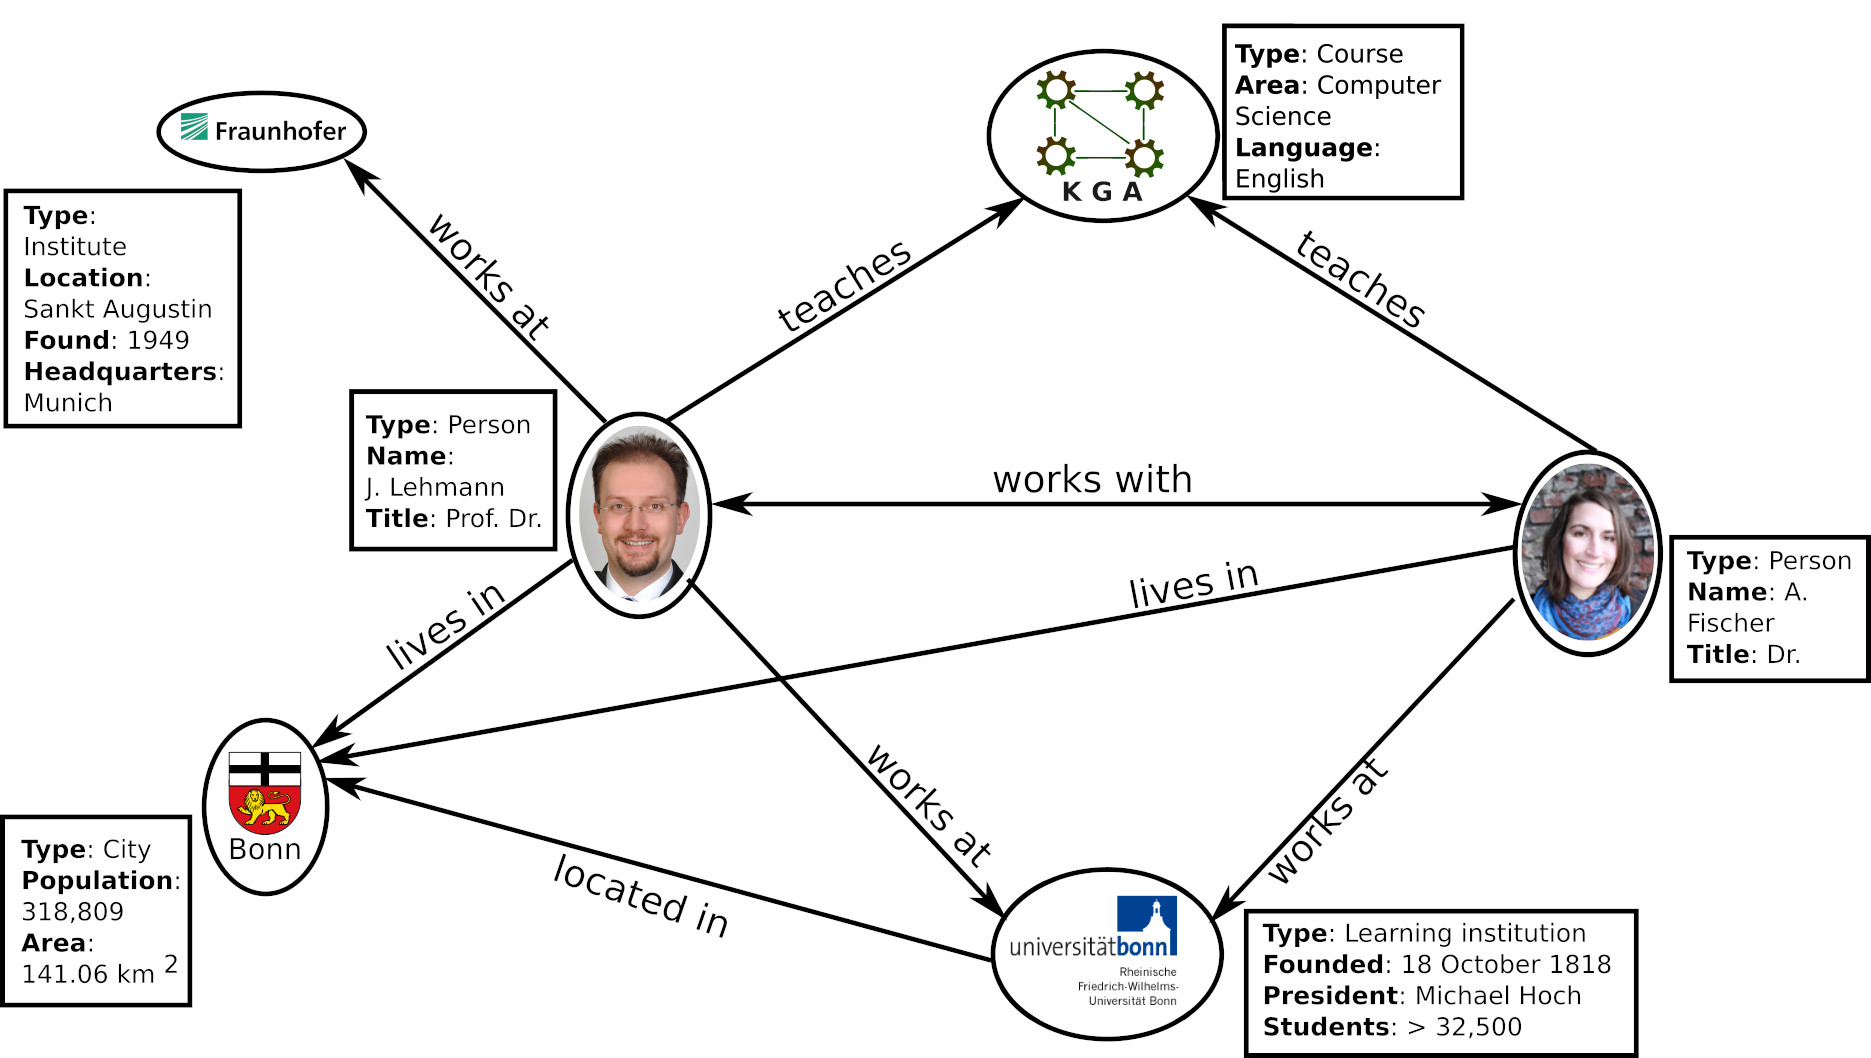
\includegraphics[width=0.8\linewidth]{know-graph-bgw}
      \end{center}
    \end{frame}    

    \begin{frame}{Grakn}
      \framesubtitle{\alert{Architecture}}%
      \begin{center}
        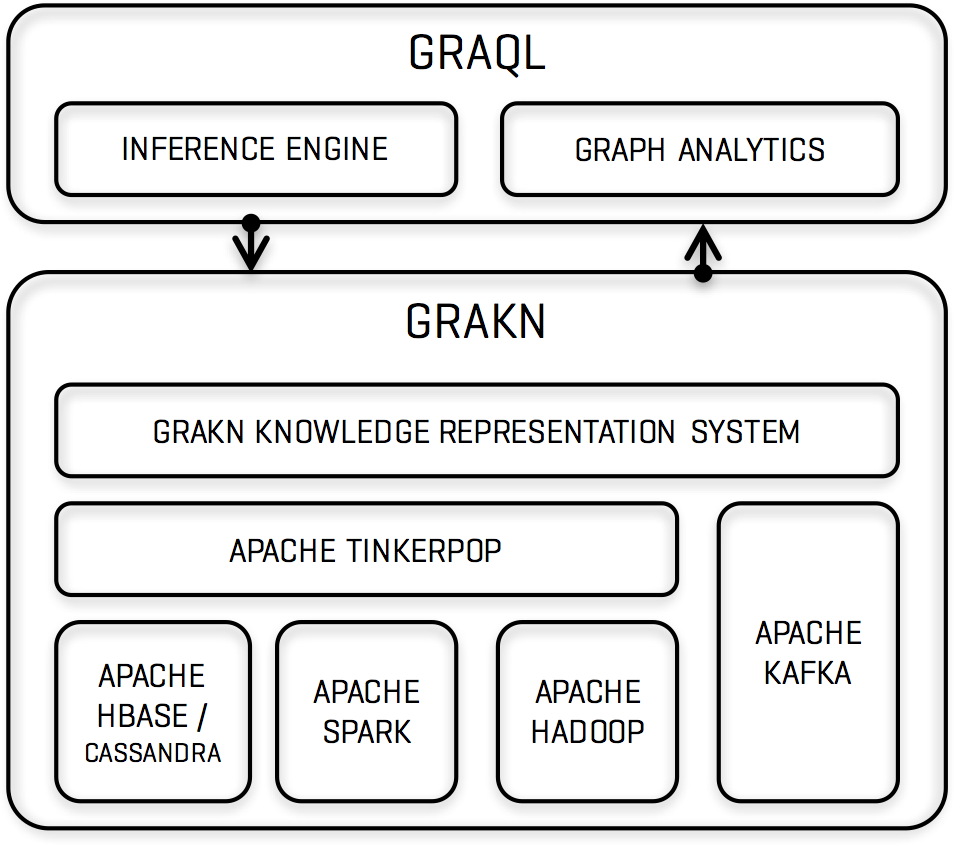
\includegraphics[width=0.5\linewidth]{architecture}
      \end{center}
    \end{frame}    

    \begin{frame}{Grakn}
      \framesubtitle{\alert{Schema}}%
      \begin{center}
        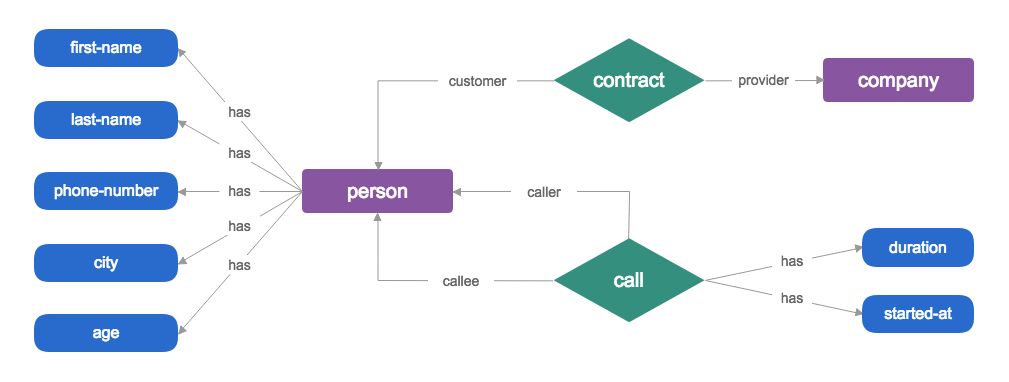
\includegraphics[width=\linewidth]{schema}
      \end{center}
    \end{frame}      
    
    \begin{frame}{Grakn}
      \framesubtitle{\alert{DDL \& DML}}%
      \begin{center}
        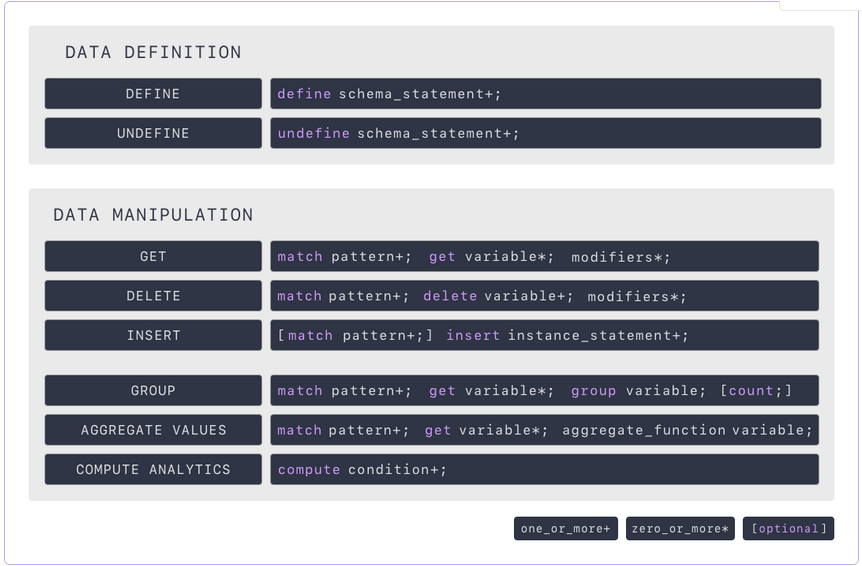
\includegraphics[width=0.6\linewidth]{dmlyddl}
      \end{center}
    \end{frame}        

    \begin{frame}{Solution}
      \framesubtitle{\alert{Types of semantic relationships}}%
      \begin{center}
        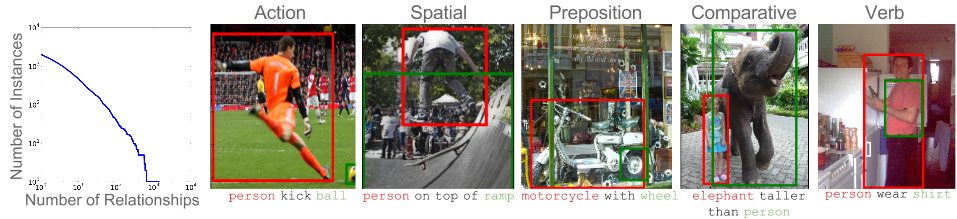
\includegraphics[width=\linewidth]{predica}
      \end{center}
    \end{frame}       

    \begin{frame}{Solution}
      \framesubtitle{\alert{Predicates of the semantic relationships types}}%
      \begin{center}
        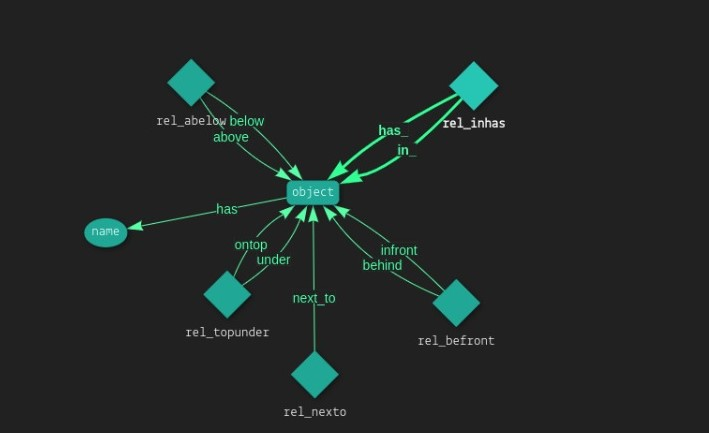
\includegraphics[width=0.8\linewidth]{dObje}
      \end{center}
    \end{frame}       
   
    \begin{frame}{Solution}
      \framesubtitle{\alert{Relationships draft}}%
      The following figure shows a draft of all the relations ships
      recover from our study object.
      % En la siguiente figura se presenta un bosquejo de las todas las 
      % relaciones de espacialidad recuperadas de nuestro objeto de estudio
      \begin{center}
        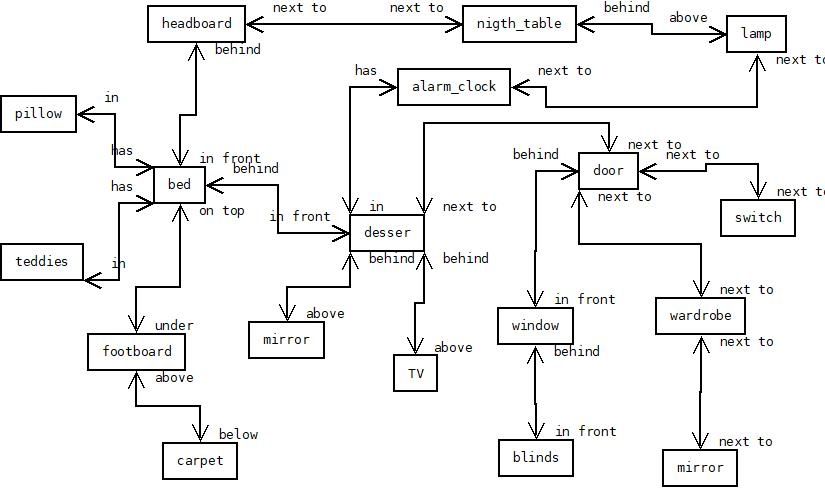
\includegraphics[width=0.7\linewidth]{grafo}
      \end{center}
    \end{frame}  

    \begin{frame}{Solution}
      \framesubtitle{\alert{Graph generate with Grakn}}%
      \begin{center}
        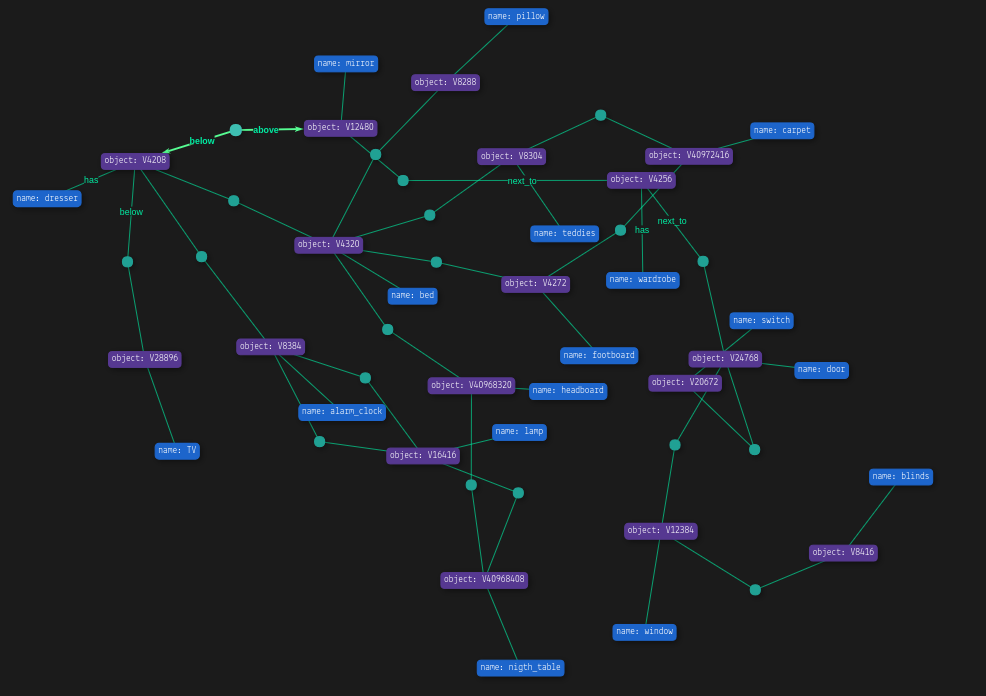
\includegraphics[width=0.7\linewidth]{allrel2}
      \end{center}
    \end{frame}   

    \begin{frame}{Solution}
      \framesubtitle{\alert{Graph generate with Grakn}}%
      \begin{center}
        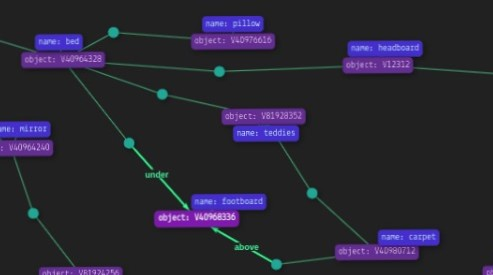
\includegraphics[width=0.85\linewidth]{realcionGrafo}
      \end{center}
    \end{frame}  

    \begin{frame}{Conclusions}
      \begin{itemize}
        \item We show that it is possible to create a knowledge graph from
        the semantic relationships that occur in an indoor space of human 
        ocuppation
        \item The most accurate predicate, in our scenario for binding two 
        objects is the \textit{spatial} relationship.
        \begin{itemize}
          \item Indeed, in most localization scenarios this predicate is the most
          accurate because the other produces so many combinations.
        \end{itemize}
        \item Grakn is a very outstading tool to create knowlegde graph with a 
        given list of predicates.
        \begin{itemize}
          \item Grakn even offers the possibility of making \textit{machine
          reasoning} from the data input.
        \end{itemize} 
        \item We seek to create complementary datasets that will help 
        convolutional layer neural network to reduce processing time.
      \end{itemize}
    \end{frame}   

  \end{darkframes}

\end{document}
